\documentclass[UTF8]{ctexbeamer}
\usetheme{Madrid}
\usecolortheme{whale}
\usepackage{hyperref}
\usepackage{graphicx}
\usepackage{wrapfig}

\DeclareGraphicsExtensions{.eps,.ps,.jpg,.bmp,.png}

\title{网络协议简介与 Linux 网络应用}

\subtitle{Down-Top Method}

\author[Linux 开源学生俱乐部]
{本群最菜 % \inst{1}
%  \and 可爱BC \inst{2}
}

\date{April 2021}

\AtBeginSection[]
{
	\begin{frame}
		\frametitle{Index}
		\tableofcontents[currentsection]
	\end{frame}
}



\begin{document}

\frame{\titlepage}
\begin{frame}
	\frametitle{Index}
	\tableofcontents
\end{frame}

\section{Data Link Layer}
\begin{frame}{Dual Computer Interconnection}
    
    \begin{figure}
        \centering
        
\includegraphics[width=0.8\textwidth]{dual-computer-interconnection.png}
        % \caption{Caption}
        % \label{fig:my_label}
    \end{figure}
    Practice: 
\end{frame}
\begin{frame}{Multiple Computer Interconnection}
    \begin{figure}
        \centering
        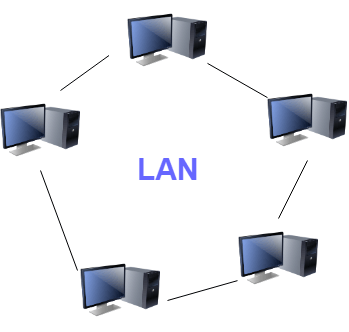
\includegraphics[width=0.6\textwidth]{lan.png}
        % \caption{Caption}
        % \label{fig:my_label}
    \end{figure}
    % https://www.guru99.com/types-of-computer-network.html
\end{frame}

\begin{frame}{Ethernet Hub}
    
    % https://commons.wikimedia.org/wiki/File:4_port_netgear_ethernet_hub.jpg
\end{frame}

\begin{frame}{Half Duplex}
    \begin{figure}
        \centering
        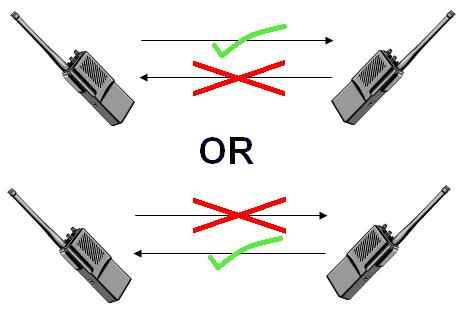
\includegraphics[width=0.6\textwidth]{HalfDuplex.jpg}
        % \caption{Caption}
        % \label{fig:my_label}
    \end{figure}
    % https://en.wikipedia.org/wiki/Duplex_(telecommunications)
\end{frame}
\begin{frame}{Full duplex}
    \begin{figure}
        \centering
        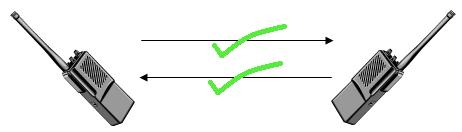
\includegraphics[width=0.6\textwidth]{FullDuplex.jpg}
        % \caption{Caption}
        % \label{fig:my_label}
    \end{figure}
    % https://en.wikipedia.org/wiki/Duplex_(telecommunications)
\end{frame}
\begin{frame}{Broadcast storm}
    % https://en.wikipedia.org/wiki/Broadcast_storm
    % https://blog.apnic.net/2019/05/28/broadcast-storms-in-service-provider-networks/
\end{frame}
\section{Network Layer}
\begin{frame}
	\frametitle{Problems with Dual Computer Interconnection}
	Difficult to extend.
   	e.g.
	\begin{figure}
	    \centering
	    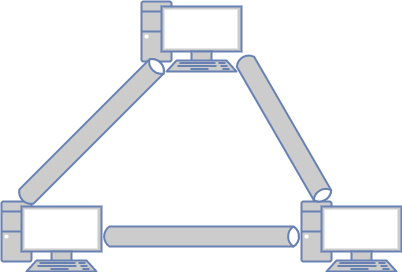
\includegraphics[width=0.25\textwidth]{extension-difficulty.png}
	    \caption{Ring Network}
	   % https://en.wikipedia.org/wiki/Star_network
   \end{figure}
   
    to extend each end it requires an additional port on all other ends.(which is unaffordable,let alone large scale network)
\end{frame}


\begin{frame}{A Solution}

    How about connecting each end to a single cable?
     \begin{figure}
         \centering
         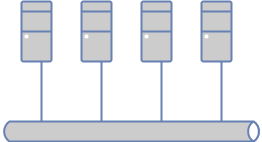
\includegraphics[width=0.4\textwidth]{Bus.png}
         \caption{Bus}
        %  \label{fig:my_label}
     \end{figure}
     In this case every single machine is connected to all other ends.
     
     The device to achieve this type of connection is a \textbf{Hub}
     
     
     
\end{frame}

\begin{frame}{A Solution}

    \begin{figure}
        \centering
        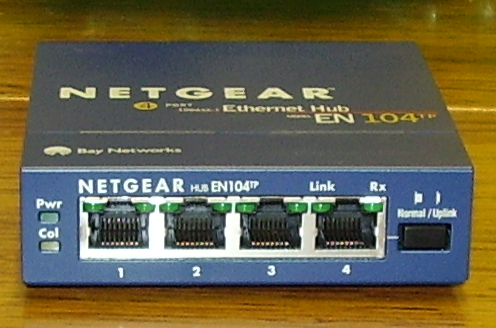
\includegraphics[width=0.8\textwidth]{4-port-netgear-ethernet-hub.jpg}
        % \caption{Caption}
        % \label{fig:my_label}
    \end{figure}
    
\end{frame}


\begin{frame}{New Problems arise}
    In this case, multiple ends communicate over the same cable.
    They need to distinguish from each other. \pause
    Let start by giving names, in Network this is called a MAC address.
    \begin{figure}
        \centering
        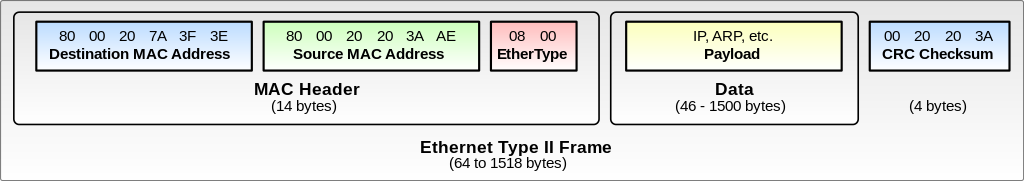
\includegraphics[width=0.6\textwidth]{Ethernet-Type-II-Frame-format.png}
        % https://en.wikipedia.org/wiki/Ethernet_frame
        % \caption{Caption}
        % \label{fig:my_label}
    \end{figure}
\end{frame}

\begin{frame}{Enlarge the scale}
    If multiple ends try sending at the same time...
    Collision.\pause
    
    Exp-Backoff.\pause
    
    But it doesn't help that much.
    % As the Network Grows and so does the comms , Collisions happen so frequently
    % that we're always backing off.
    % The speed is double-downed.
    
\end{frame}

\begin{frame}{Upgrading the Hub}
    There was a simple idea.What if we separate the ends from a single wire?
    We can achieve this by applying some upgrades to the Hub.
    Enpower the hub with memory to avoid broadcasting to all ends in the network.
    \begin{figure}
        \centering
        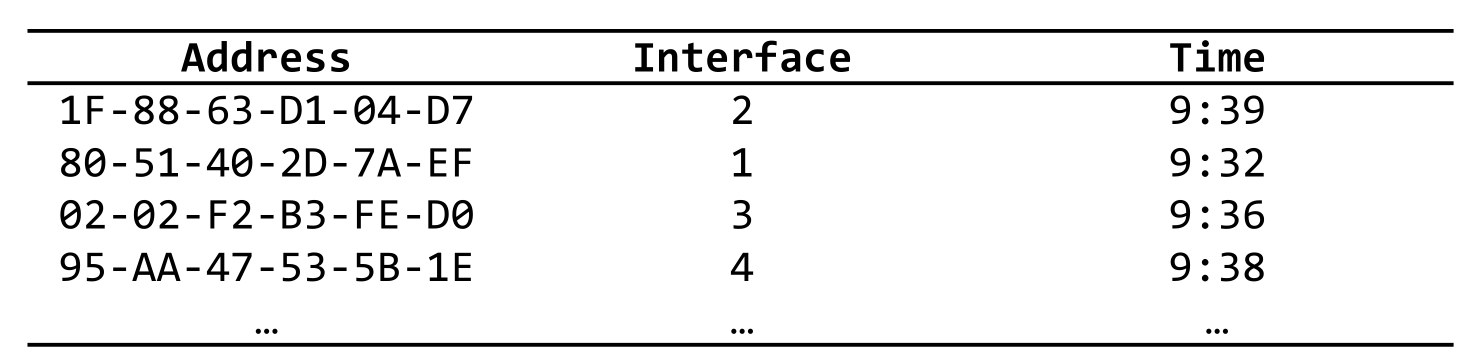
\includegraphics[width=0.6\textwidth]{mac-table.png}
        \caption{Mac Table}
        % \label{fig:my_label}
    \end{figure}
        \begin{figure}
        \centering
        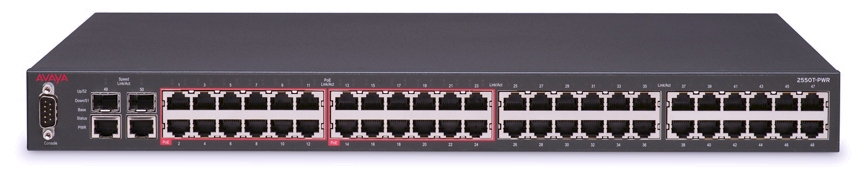
\includegraphics[width=0.6\textwidth]{2550T-PWR-Front.jpg}
        \caption{Switch}
        % \label{fig:my_label}
    \end{figure}

\end{frame}

\begin{frame}[fragile]{The Behaviour of the Switch}
% \begin{onlyenv}<2>
% \begin{minted}{python}
\begin{verbatim}
for each Port A:
  for each MAC frame it received on Port A:
    lookup the Switch Table
    if found:
      if it belongs to Port A itself:
        do nothing 
      else:
        Forward The MAC frame to corresponding Port
    else:
      Broadcast the Frame to all other Port except A
\end{verbatim}
% \end{minted}
% \end{onlyenv}
\end{frame}

\begin{frame}{The Problem Still Exists}
    In the status quo, Consider a large-scale network.
    \begin{figure}
        \centering
        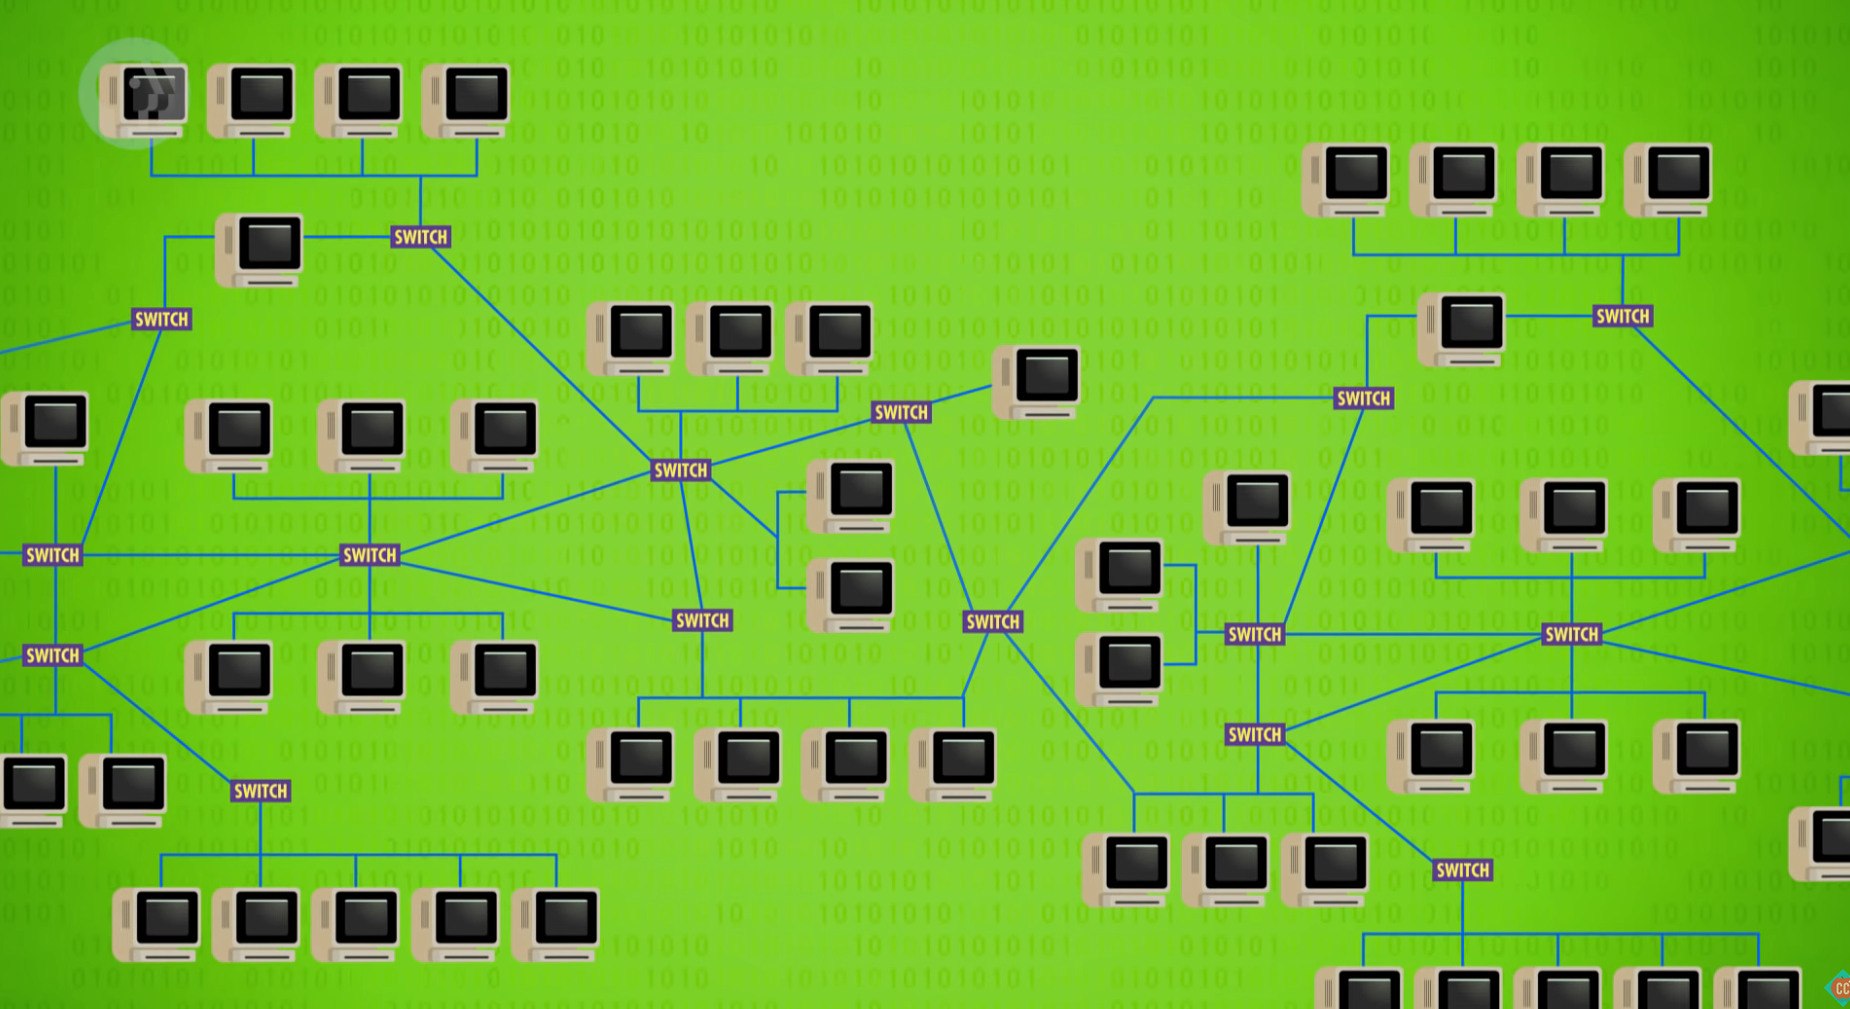
\includegraphics[width=0.8\textwidth]{large-scale-ethernet.png}
        \caption{Burdened Switch}
        % \label{fig:my_label}
    \end{figure}
    
\end{frame}

\begin{frame}{A closer look}
    For each Switch,we notice that in order to Send MAC frames to a far end it needs to maintain too much information (and we must,Why?)
    \begin{figure}
        \centering
        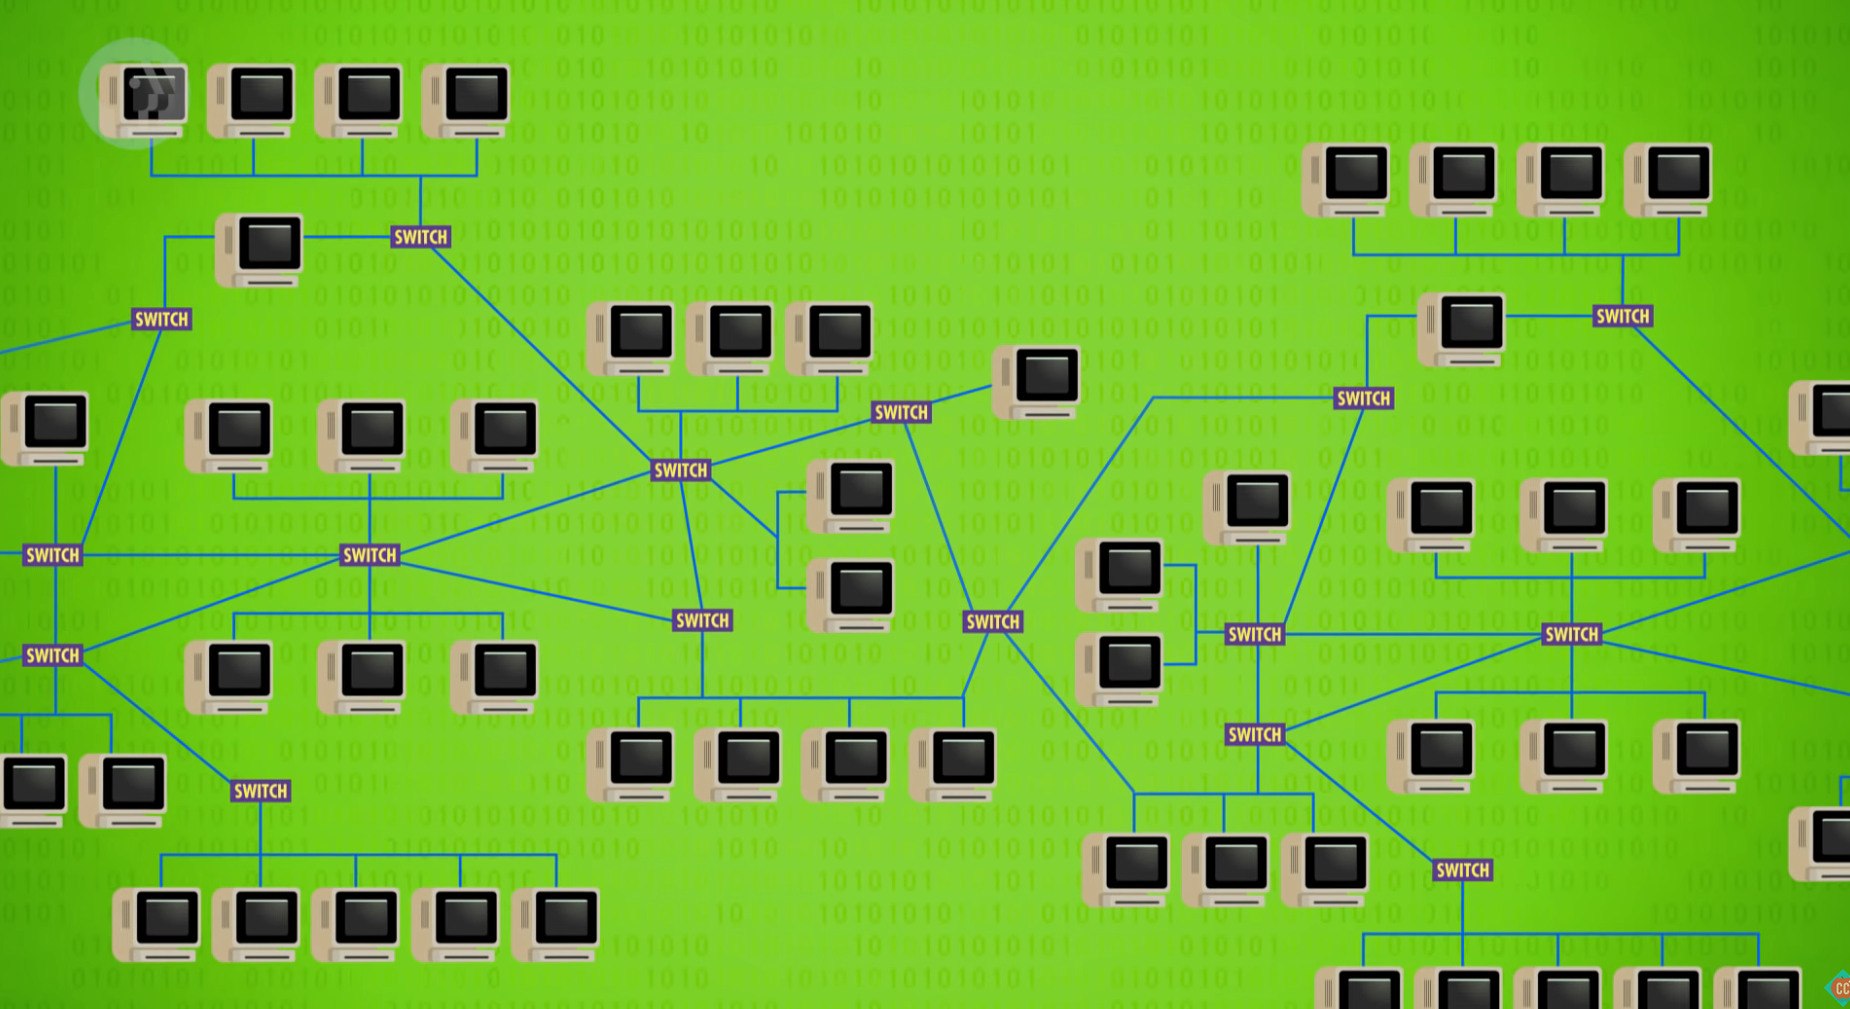
\includegraphics[width=0.8\textwidth]{large-scale-ethernet.png}
        \caption{Burdened Switch}
        % \label{fig:my_label}
    \end{figure}
    
\end{frame}

\begin{frame}{Router}
    \begin{figure}
        \centering
        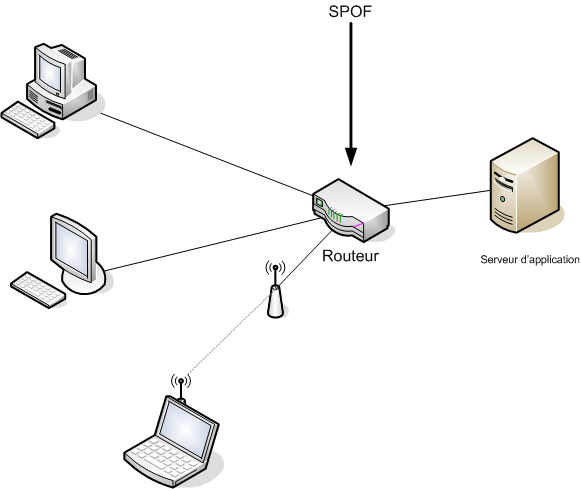
\includegraphics[width=0.6\textwidth]{SPOF.png}
        % https://zh.wikipedia.org/wiki/%E8%B7%AF%E7%94%B1%E5%99%A8
        % \caption{Caption}
        % \label{fig:my_label}
    \end{figure}
\end{frame}

\begin{frame}{IP Protocol}
    \begin{figure}
        \centering
        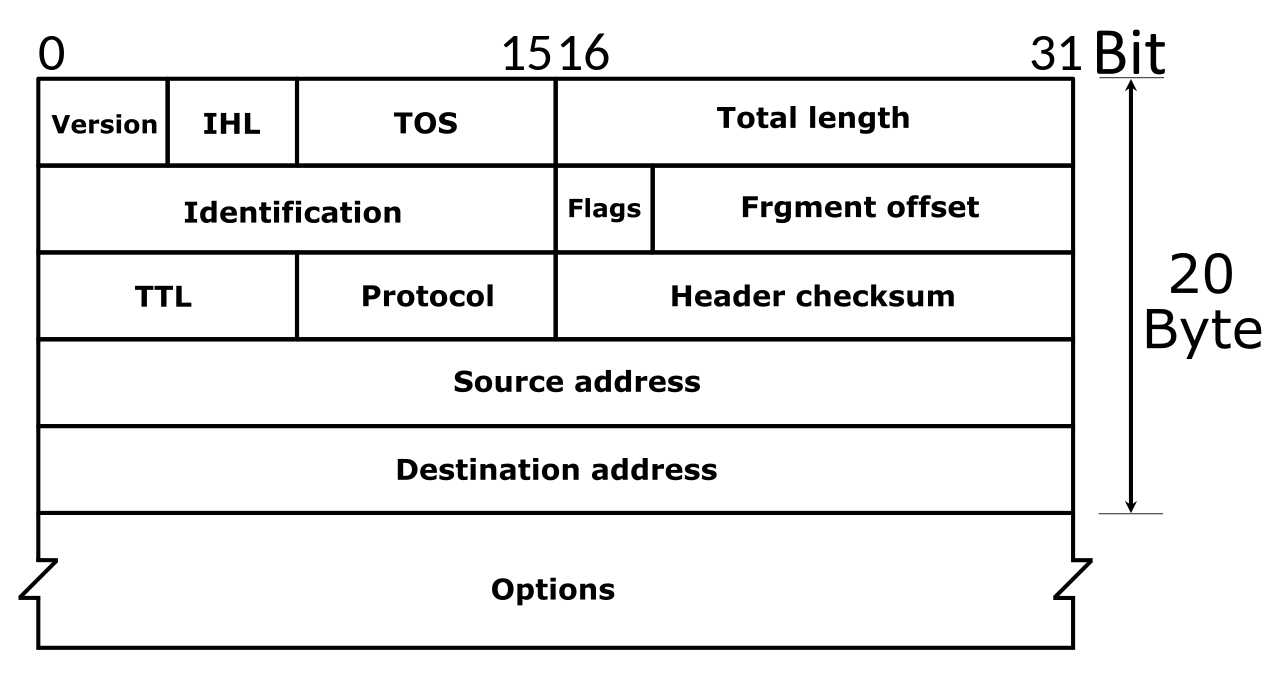
\includegraphics[width=0.5\textwidth]{IPv4_Header.png}
        % \caption{Caption}
        % \label{fig:my_label}
    \end{figure}
    \begin{figure}
        \centering
        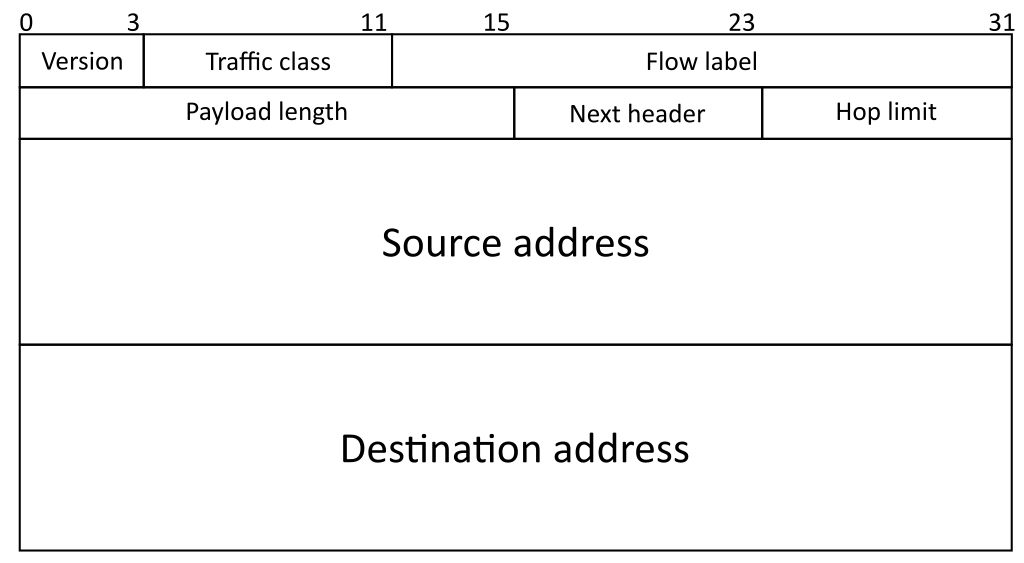
\includegraphics[width=0.5\textwidth]{IPv6_Header.png}
        % \caption{Caption}
        % \label{fig:my_label}
    \end{figure}
\end{frame}

\begin{frame}{IPv4 Address}
    32-bit number
    
    four 8-bit fields that are separated by periods
    
    192.168.1.1
\end{frame}

\begin{frame}{IPv4 CIDR}
    Classless Inter-Domain Routing
    
    Ex.
    
    192.168.1.0/24 equals 192.168.1.0 - 192.168.1.255
    
    192.168.0.0/23 equals 192.168.0.0 - 192.168.1.255
    
    10.0.0.0/8 equals 10.0.0.0 - 10.255.255.255
    
    \url{https://en.wikipedia.org/wiki/Classless\_Inter-Domain\_Routing\#IPv4\_CIDR\_blocks}
\end{frame}

\begin{frame}{Router}
    A router is a networking device that forwards data packets between computer networks.
    
    \vspace{5mm}
    
    A router is connected to two or more data lines from different IP networks.
    
    \vspace{2mm}
    
    When a data packet comes in on one of the lines, the router reads the network address information in the packet header to determine the ultimate destination. Then, using information in its routing table or routing policy, it directs the packet to the next network on its journey.
    % https://en.wikipedia.org/wiki/Router_(computing)
\end{frame}

\begin{frame}{ARP\footnotemark}
    The address resolution protocol is a protocol used by the IP, specifically IPv4, to map IP network addresses to the hardware addresses used by a data link protocol.
    % https://erg.abdn.ac.uk/users/gorry/course/inet-pages/arp.html
    \begin{figure}
        \centering
        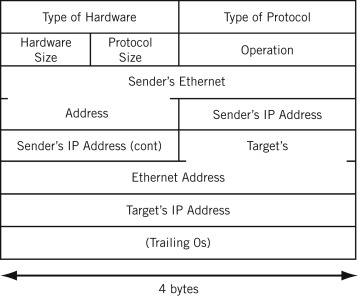
\includegraphics[width=0.4\textwidth]{arp.jpg}
        % https://www.sciencedirect.com/topics/computer-science/address-resolution-protocol-request
        % \caption{ARP}
        % \label{fig:my_label}
    \end{figure}
    \begin{itemize}
        \item ARP-Request (Broadcast, source IP address of the requester)
        \item ARP-Reply (Unicast to requester, the target)
    \end{itemize}
    \footnotetext[1]{In IPv6, NDP is used instead}
\end{frame}

\begin{frame}{To Be more intuitive}
\begin{figure}
    \centering
    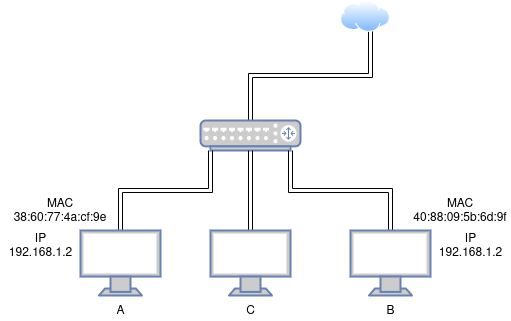
\includegraphics[width=0.5\textwidth]{ARP.png}
\end{figure}
Host A wants to communicate with IP 192.168.1.4,After checking the routing table which says this address requires no routing,
but A doesn't know the MAC of IP 192.168.1.4.

Host A:(Broadcast) Who is 192.168.1.4?Please Respond to MAC 38:60:77:4a:cf:9e

Host B:(To A's MAC) This is 192.168.1.4

Host A:[Taking notes]and after some time,A refreshes this 'note'

    
\end{frame}

\begin{frame}{Kernel IP routing table}
    \begin{figure}
        \centering
        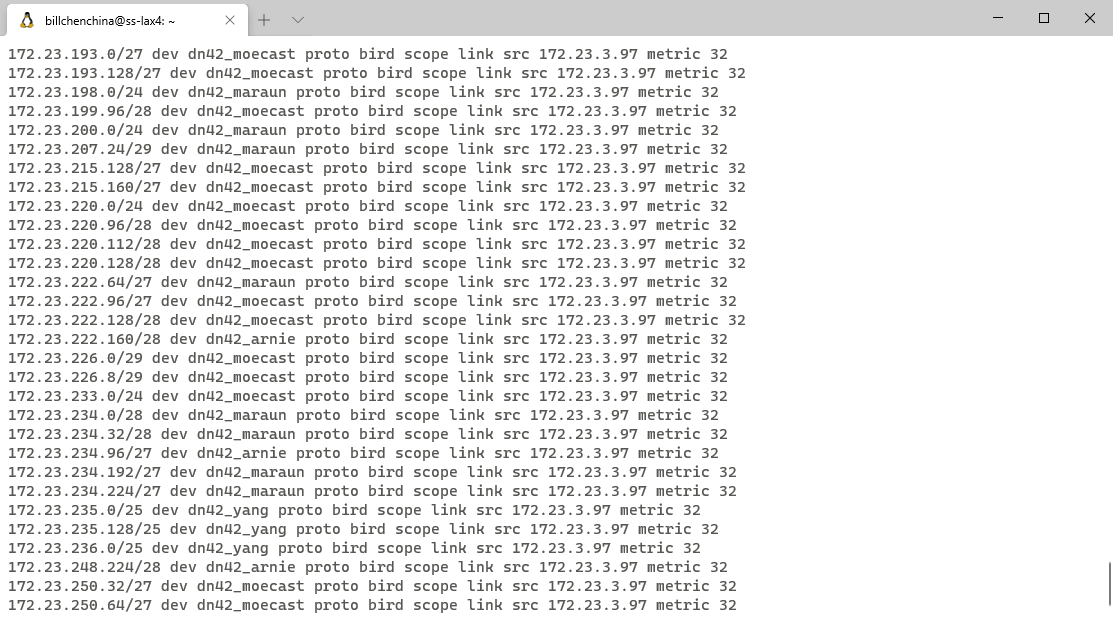
\includegraphics[width=0.7\textwidth]{linux-routing-table.png}
        \caption{Linux Routing Table}
        % \label{fig:my_label}
    \end{figure}
    % netstat -nr
    % ip route
    % https://tldp.org/LDP/nag/node75.html
\end{frame}

\begin{frame}[fragile]{Manipulating routing table}
e.g.
\begin{verbatim}
ip route show
ip route add <CIDR> [via IP] dev <interface>
ip route del <CIDR> [via IP] dev <interface>
\end{verbatim}
    
    
\end{frame}

\begin{frame}[fragile]{Multi-Table Routing}
e.g.
% http://linux-ip.net/html/routing-tables.html
\begin{verbatim}
ip route add <CIDR> [via IP] dev <interface> table <table_id>
ip rule show
ip rule add fwmark lookup <table id>
ip rule del 
\end{verbatim}
  
    
\end{frame}
\begin{frame}{iptables}
    \begin{figure}
        \centering
        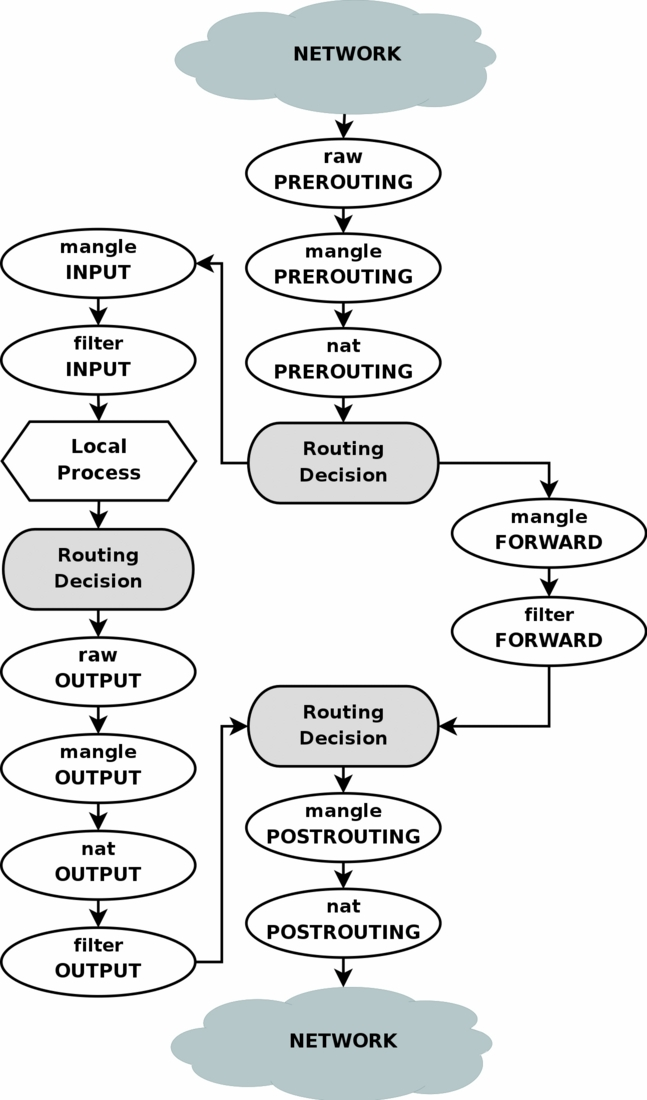
\includegraphics[height=0.5\textwidth]{tables_traverse.jpg}
        \caption{iptables}
        % \label{fig:my_label}
    \end{figure}
    % https://www.frozentux.net/iptables-tutorial/iptables-tutorial.html#TRAVERSINGOFTABLES
\end{frame}
\end{document}
